\subsection{Vision Detection Principles}

The task was to identify the model of the card from the variations on shape, shape count and the filler. Figure shows the different variables in the used card set.

	\begin{figure}[position = here]
		\begin{centering}
			
\includegraphics[scale=0.5]{./sachiths_images/image123.png}\\
			\caption[]{\textit{Different types of cards}}
		\end{centering}
	\end{figure}
	\begin{figure}
		\centering
		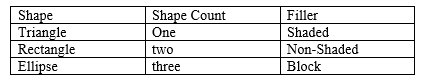
\includegraphics[scale=0.8]{./sachiths_images/image2.png}
		\caption[]{\textit{Variables}}
	\end{figure}

In the robot arm we had there is a camera mounted on top of the table which can be used to get images of the objects place on the table. This images can be used to identify the object properties using image processing techniques. 

There are plenty of approaches to find features in image processing. Following are some of the processing techniques.


\begin{enumerate}
	\item Edge detection.
	\item Corner detection.
	\item Hough transformation.
	\item Swift operator.
	\item Binary image processing
	\item Histogram comparisons. \ldots
\end{enumerate}

In this project Edge detection and Binary image processing methods have been used to identify the cards from the table and shapes in the cards.

\textbf{Edge detection}

An edge in an image is a significant local change in the image intensity, usually associated with a discontinuity in either the image intensity or the first derivative of the image intensity. Matlab toolbox has an inbuilt function for Edge detection. Canny operator have been used in this project.

\textbf{Binary image processing}

Thresholding: Using the histogram of the image a threshold can be identified to convert the image to a binary image with areas of interests. This method was feasible to this project as the image of back of the card gives pixel value near to black and a image of the front of the card gives pixel values near to white.

Position/Orientation: After creating the binary image with interested regions matlab inbuilt functions can be used to identify centroids and orientations of the interested regions. Local positions can be transferred to world coordinates using a reference point in this case are 3 fiducial boxes at known positions.


%%%%%%

%{3}
%\bibitem{Canny}
%John Canny, \emph{Pattern Analysis and Machine Intelligence  },6th~ed\hskip 1em plus
%0.5em minus 0.4em\relax IEEE, 1986/11.

%{2}
%\bibitem{Edge}
%R.Jain,R Kasturi,B.G.Schucnk \emph{Machine Vision}, 1st~ed\hskip 1em plus
%0.5em minus 0.4em\relax McGraw-Hill,Inc, 1995.